\chapter{\TeX のサンプル}\label{sample}

\section{ラベルのはりかた}\label{sec:label}
label命令で名前をつける.\TeX では章節や図の番号は自動で振られるので,label命令でつけた名前にref命令でアクセスして番号を取得する.
例としてこの章は,第\ref{sample}章,など.

\subsection{サンプル一覧}\label{sec:list}
ラベルの貼り方(\ref{sec:label}),数式のいれかた(\ref{sec:eq}),図のいれかた(\ref{sec:figure}),表のいれかた(\ref{sec:table}),参考文献の付け方(\ref{sec:ref})など.

\section{数式のいれかた}\label{sec:eq}
数式が美しく組版されるのは\TeX を使う主要な理由の一つである.\TeX の数式には行内に入れる数式(例$E=mc^2$)と別行立ての数式,

\begin{equation}
	\label{eq:test1}
	E = \sqrt{m^2 c^4 +|\bm{p}|^2 c^2}
\end{equation}

がある.
数式番号を入れたくなければ,
\begin{equation}
	\nonumber
	\label{eq:test1}
	E = \sqrt{m^2 c^4 +|\bm{p}|^2 c^2}
\end{equation}

複数行にわたる式で,位置を揃えたければ,
\begin{eqnarray}
	\nonumber
	E & =    & \sqrt{m^2 c^4 +|\bm{p}|^2 c^2} \\
	  & \sim & mc^2
\end{eqnarray}

とする.

\section{図のいれかた}\label{sec:figure}

一般に図はpdfファイル或いはjpgファイルで用意するのが良い.
pdfファイルでもjpgファイルでもいれかたは同じ.
図を入れたいところに入れようとしないこと.
適切な位置に挿入するのは\TeX 様がやってくれる.


\begin{figure}[tb]
	\centering
	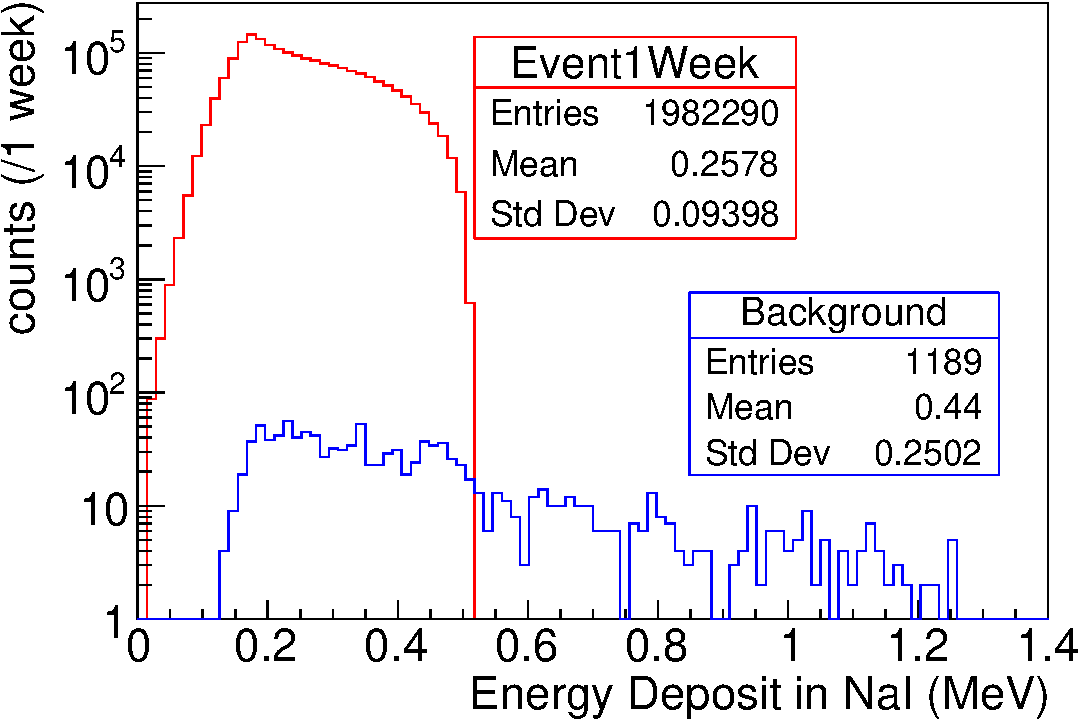
\includegraphics[width=10cm]{fig/figure.pdf}
	\caption{適当な図}
	\label{fig:test1}
\end{figure}

\begin{figure}[tb]
	\centering
	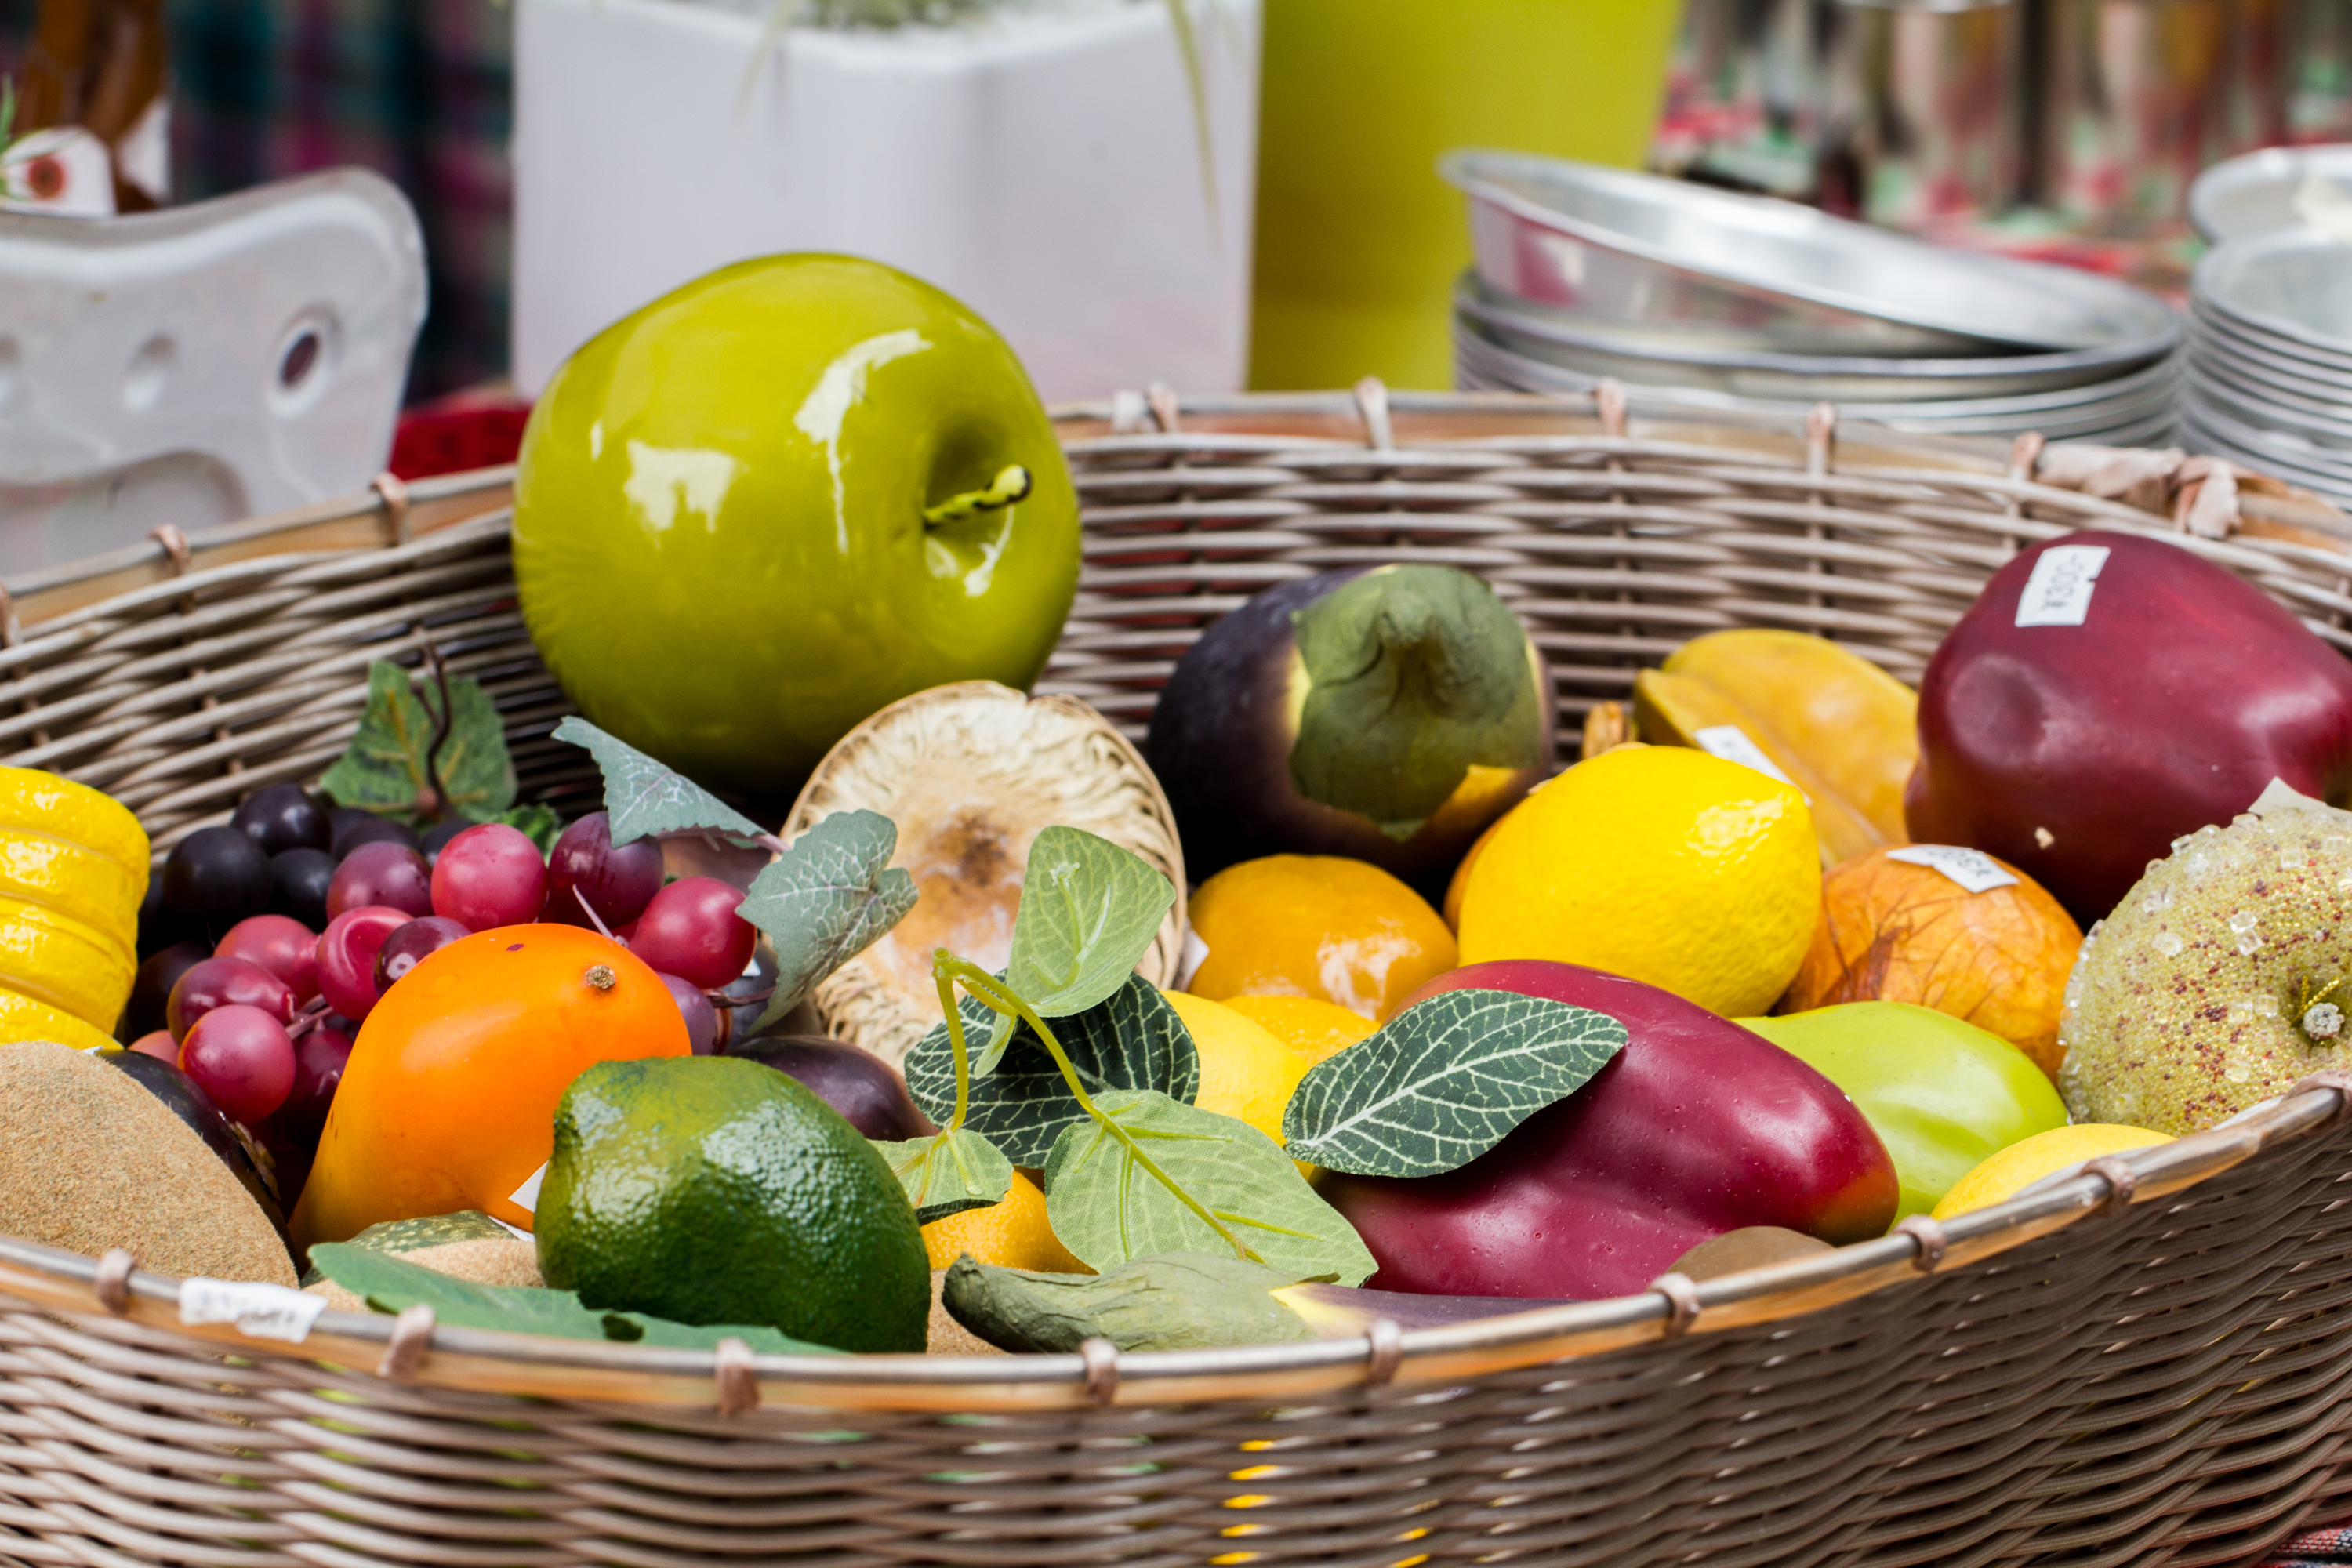
\includegraphics[width=10cm]{fig/image.jpg}
	\caption[ここが目次の図タイトル]{本文の図タイトル \newline すごく長くこの図の説明をしたければ長く書くだけ適当にインデントされる.}
	\label{fig:test2}
\end{figure}

図\ref{fig:test3}と図\ref{fig:test4}は横に並べたいときの例.

\begin{figure}[tb]
\begin{tabular}{cc}
\centering

\begin{minipage}{0.5\hsize}
	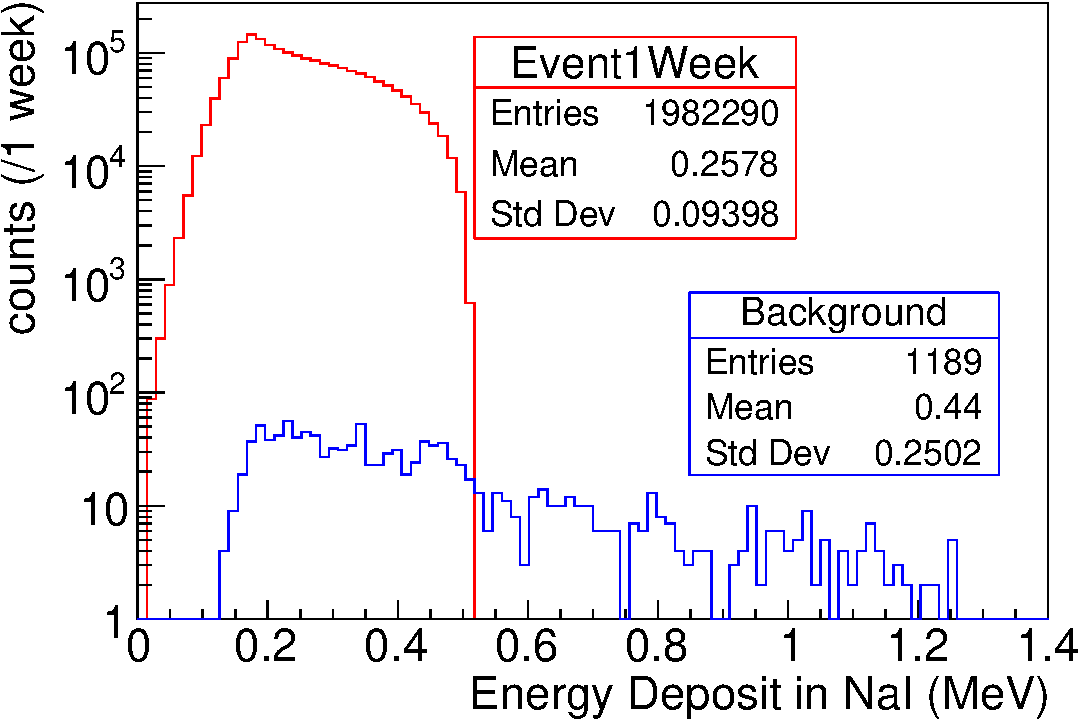
\includegraphics[width=7cm]{fig/figure.pdf}
	\caption{左の図}
	\label{fig:test3}
\end{minipage}&

\begin{minipage}{0.5\hsize}
	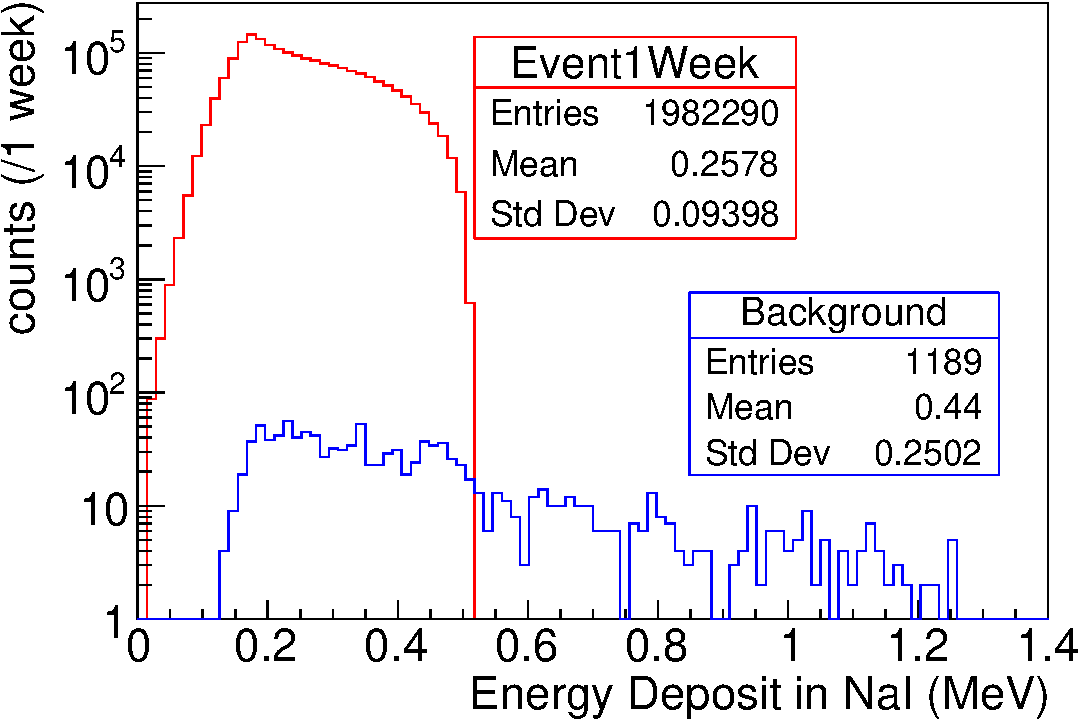
\includegraphics[width=7cm]{fig/figure.pdf}
	\caption{右の図}
	\label{fig:test4}
\end{minipage}

\end{tabular}
\end{figure}


\section{表のいれかた}\label{sec:table}

表は以下の書式で作成する.サンプルを表\ref{tab:test5}に示す.
\begin{table}[tb]
	\centering
	\caption{表の例}
		\label{tab:test5}	
	  \begin{tabular}{lcc} 
		\hline
		 		&信号& バックグラウンド \\ 
		\hline \hline
		例1 	& 1	 & 40,000			\\
		例2 	& 2  & 50,000			\\
		例3 	& 3  & 60,000			\\
		\hline
	  \end{tabular}
\end{table}

\section{引用のしかた}\label{sec:ref}
bibファイルをArXiVなりLead2Amazonなりからとってきて,reference.bibに取り込む.
本文中ではciteで自動的にリファレンスが作成される\cite{myThesisTest1}.
複数個つけることもできる\cite{myThesisTest2,myWebsite}.


